\documentclass[aspectratio=169]{beamer}

\usepackage[utf8]{inputenc}
\usepackage{booktabs}
\usepackage[UKenglish,russian]{babel}
\usepackage{epigraph}
\usepackage{hyperref}
\usepackage{csquotes}
\usepackage{tcolorbox}
\usepackage{multicol}
\usepackage{braket}
\usepackage{booktabs}
\usepackage[ruled, linesnumbered, algo2e]{algorithm2e}

\usecolortheme{seahorse}
\beamertemplatenavigationsymbolsempty

\setbeamertemplate{footline}{%
\hfill\usebeamertemplate***{navigation symbols}
\hspace{1cm}\insertframenumber{}/\inserttotalframenumber}

\setlength\algotitleheightrule{0pt}
\SetKwInOut{Input}{Frage}


\RequirePackage{amsmath}
\RequirePackage{amssymb}
\RequirePackage{tikz}
\usetikzlibrary{
    arrows,
    decorations.pathmorphing,
    decorations.pathreplacing,
    calligraphy,
    positioning,
    matrix, 
    patterns,
    automata,
    calc,
    tikzmark}

\renewenvironment{definition}{
    \begin{tcolorbox}[
        title=Definition, 
        sharp corners, 
        colback=white, 
        boxrule=0.4pt, 
        colframe=violet]
}{
    \end{tcolorbox}
}

\renewenvironment{theorem}{
    \begin{tcolorbox}[
        title=Satz, 
        sharp corners, 
        colback=white, 
        boxrule=0.4pt, 
        colframe=violet]
}{
    \end{tcolorbox}
}
\setbeamercolor{alerted text}{fg=violet!60!white}

\newcommand{\fullyConnected}[2]{
    \begin{tikzpicture}
        \foreach \x in {0,#1,...,359} {
            \node[draw,circle,fill=#2] (v\x) at (\x:.75) {};
        }
        \foreach \x in {0,#1,...,359} {
            \foreach \y in {0,#1,...,359}{
                \draw (v\x) -- (v\y);
            }
        }
        \node[white] at (0:.75) {$t$};
        \node[white] at (#1:.75) {$s$};
    \end{tikzpicture}
}

%===============================================
% Problems and Complexity Classes
%===============================================

\newcommand{\leqlm}{\mathrel{\leq^{\log}_{\text m}}}

\newcommand{\class}[1]{\ensuremath{\mathrm{#1}}\xspace}
\newcommand{\prblem}[1]{\ensuremath{\mathsf{#1}}\xspace}

\newcommand{\SPACE}{\class{SPACE}}
\newcommand{\NSPACE}{\class{NSPACE}}
\newcommand{\TIME}{\class{TIME}}

\newcommand{\LSPACE}{\class{L}}
\newcommand{\NL}{\class{NL}}
\newcommand{\LOGCFL}{\class{LOGCFL}}
\newcommand{\AC}{\class{AC^1}}
\newcommand{\DP}{\class{P}}


\newcommand{\GAP}{\prblem{GAP}}
\newcommand{\AGAP}{\prblem{AGAP}}
\newcommand{\ASGAP}{\prblem{ASGAP}}

\DeclareMathOperator{\apath}{apath}
\newcommand{\discup}{\mathbin{\dot \cup}}

\newcommand{\IG}{\mathrm{IG}}
\newcommand{\DBG}{\mathrm{DBG}}

\title{Research Project: A Graph Representation for Databases}
\author{Arne Meier\\(\url{meier@thi.uni-hannover.de})}
\date{13.6.2022}

\begin{document}

\begin{frame}[noframenumbering, plain]
    \maketitle
\end{frame}

\begin{frame}{But, first: Ласкаво просимо!}
    \begin{center}
    	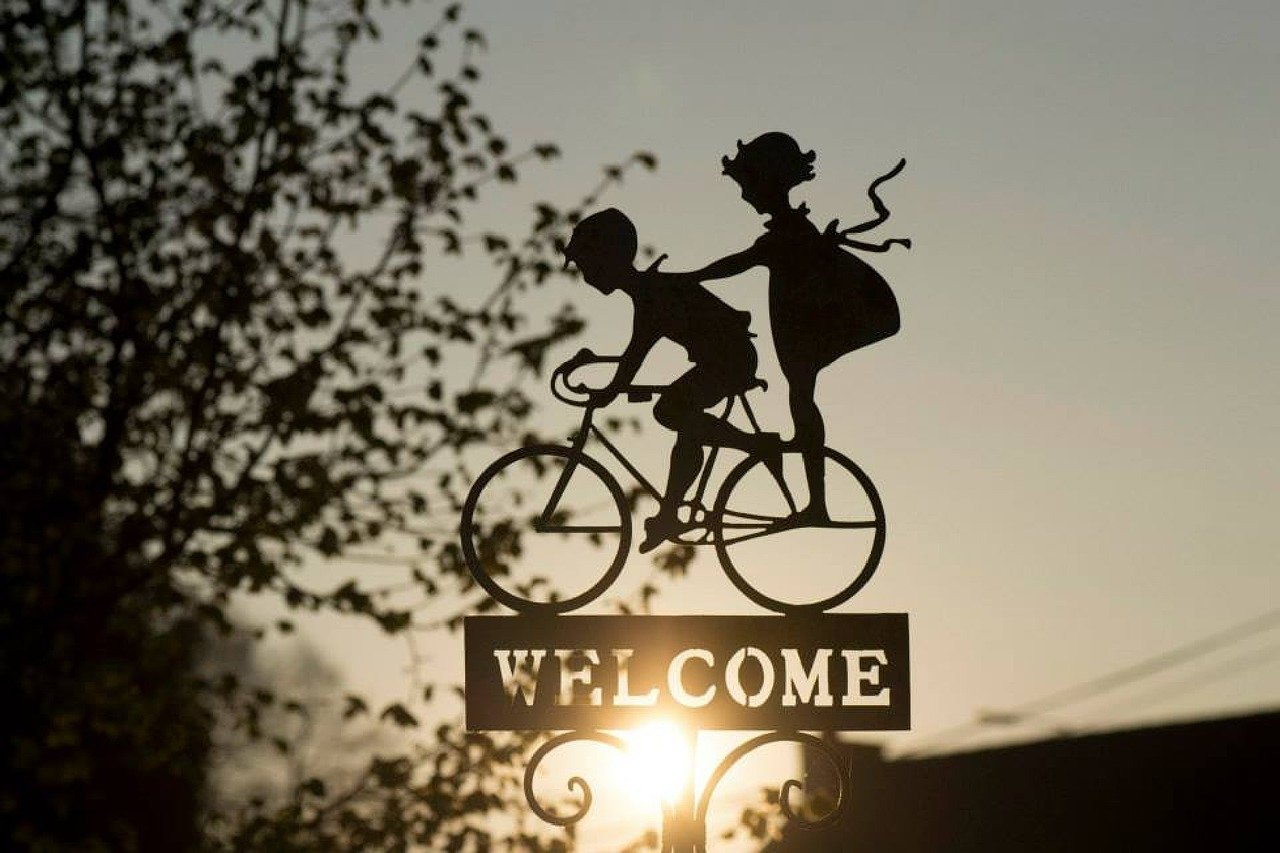
\includegraphics[width=.8\linewidth]{sign-741813_1280.jpg}
    \end{center}
\end{frame}

\begin{frame}{Regarding the Project}

\textbf{Abilities / Knowledge (you should have)}
\begin{itemize}
	\item Programming knowledge (Java, JDK $\ge$1.8)
	\item A bit of databases knowledge
	\item Propositional logic
	\item Graphs
\end{itemize}

\textbf{Also: a laptop/computer is needed}

\end{frame}

\begin{frame}{Rough Outline of the Project}
\textbf{Write in the team a program that does the following:}
\begin{enumerate}
	\item<+-> Take a propositional logic formula $\varphi$
	\item<+-> Compute its incidence graph $\IG(\varphi)$
	\item<+-> Determine the tree-width $k_\varphi\in\mathbb N$ of $\IG(\varphi)$
	\item<+-> Translate $\varphi$ into a database table $D_\varphi$
	\item<+-> Compute its database graph representation $\DBG(D_\varphi)$
	\item<+-> Determine the tree-width $\ell_\varphi\in\mathbb N$ of $\DBG(D_\varphi)$
\end{enumerate}\bigskip

\uncover<+->{\textbf{My motivating question:}
\begin{center}
	How does $\ell_\varphi$ relate to $k_\varphi$ in general?
\end{center}}
\end{frame}


\begin{frame}[fragile]{Step 1: Which propositional formulas shall we use?}
\begin{itemize}
	\item max. 500 Variables (at first: start with fewer and try how it scales)
	\item get them from \url{https://www.cs.ubc.ca/~hoos/SATLIB/benchm.html}
	\item standard format: $(x_1\lor x_3\lor \lnot x_4)\land (x_4)\land (x_2\lor \lnot x_3)$ goes to
\begin{center}
	\begin{verbatim}
c Example comment
p cnf 4 3
1 3 -4 0
4 0 2
-3	
	\end{verbatim}
\end{center}
\alert{So...} Start with writing a parser first.
\end{itemize}
\end{frame}

\begin{frame}{Step 2: Incidence Graph of Formulas}
$(u\lor\lnot v\lor\lnot y)\land(\lnot u\lor z)\land(v\lor\lnot w)\land(w\lor\lnot x)\land(x\lor y\lor\lnot z)$

becomes

\begin{minipage}{.4\linewidth}
\begin{tikzpicture}[every node/.style={inner sep=.5mm,font=\Large}]

 \node (C2) at (0,0) {$C_2$};
 \node (z) at (-1,-.5) {$z$};
 \node (u) at (1,-.5) {$u$};
 \node (C5) at (-1.5,-1.5) {$C_5$};
 \node (C1) at (1.5,-1.5) {$C_1$};
 \node (y) at (0,-1.5) {$y$};
 \node (x) at (-1.5,-2.5) {$x$};
 \node (v) at (1.5,-2.5) {$v$};
 \node (C4) at (-1,-3.5) {$C_4$};
 \node (C3) at (1,-3.5) {$C_3$};
 \node (w) at (0,-4.5) {$w$};

\foreach \f/\t in {C2/z,z/C5,C5/x,x/C4,C4/w,w/C3,C3/v,v/C1,C1/u,u/C2,C5/y,y/C1}
 \path[-,draw,black,thick] (\f) edge (\t);
\end{tikzpicture}
\end{minipage}
\begin{minipage}{.55\linewidth}
	\begin{itemize}
		\item each variable becomes a vertex
		\item each clause number becomes a vertex
		\item draw edges between clauses and their vertices
	\end{itemize}
\end{minipage}
\end{frame}

\begin{frame}[fragile]{Step 2.5: How to Represent Graphs?}
\textbf{short answer:} \url{https://pacechallenge.org/2017/treewidth/}

\begin{center}
	\begin{verbatim}
c path with five vertices and four edges.
p tw 5 4
1 2
2 3
3 4
4 5
	\end{verbatim}
\end{center}
\end{frame}


\begin{frame}{Step 3: Treewidth, Definition}
	\begin{definition}
The \alert{tree-decomposition} of a given graph $G=(V,E)$ is a tree $T=(B,E_T)$ such that: 
\begin{itemize}
	\item $\bigcup_{b\in B}=V$,
	\item for every $\{u,v\}\in E$ there is a bag $b\in B$ with $u,v\in b$ and
	\item for all $v\in V$ the restriction of $T$ to $v$ is connected.
\end{itemize}

\alert{Width} of a given tree-decomposition $T=(B,E_T)$ is $\max_{b\in B}|b|-1$.

The \alert{treewidth} of a given graph $G$ is the minimum over all widths of tree-decompositions of $G$.
\end{definition}

\end{frame}


\begin{frame}{Step 3: Treewidth, Example}
\begin{center}
\begin{minipage}{0.50\linewidth}
\begin{tikzpicture}[gate/.style={inner sep=1mm,draw,rounded corners,rectangle},scale=.75]
		\node (x0) at (0,0) {$0$};
		\node (x1) at (2,0) {$1$};
		\node (x2) at (4,0) {$2$};
		\node (x3) at (2,2) {$3$};
		\node (x4) at (4,2) {$4$};
				
		
		\foreach \f/\t in {x0/x1,x1/x2,x3/x4, x1/x3}{
			\draw[-] (\f) -- (\t);
		}
	\end{tikzpicture}
		
\end{minipage}
\begin{minipage}{0.4\linewidth}
\begin{tikzpicture}[scale=0.85, level distance= 4 em, sibling distance= 5.5 em,
	every node/.style={draw, circle, scale=0.8},
	edge from parent/.style={thin,-,black, draw}]
\node  {\textcolor{black}{$0,1$}}
	child {node {$1,3$} 
		child {node {$3,4$}}
		child {node {$1,2$}}};
\end{tikzpicture}	
\end{minipage}
\end{center}
\end{frame}

\begin{frame}{Step 3: Treewidth, Bad News}
\begin{definition}
\begin{description}
 \item[Problem] TW (Treewidth Problem)
 \item[Instances] Graph $G=(V,E)$, natural number $k\in\mathbb N$
 \item[Question] Does $G$ have a treewidth of $k$?
\end{description}
\end{definition}
This problem is NP-complete.
\end{frame}

\begin{frame}{Step 3: Treewidth, Silver Lining}
\begin{itemize}
	\item Use a blackbox for it
	\item \url{https://github.com/twalgor/tw}
\end{itemize}
\end{frame}

\begin{frame}{Step 4: Translate a Formula into a Database}
$(x_1\lor x_3\lor \lnot x_4)\land (x_4)\land (x_2\lor \lnot x_3)$ becomes two tables

$$\begin{array}{ccc}\toprule
		c & v & s \\\midrule
		C_1 & 1 & +\\
		C_1 & 3 & +\\
		C_1 & 4 &-\\
		C_2 & 4 &+\\
		C_3 & 2 &+\\
		C_3 & 3 &-\\\bottomrule
\end{array}\qquad
\begin{array}{cc}\toprule
		v & s \\\midrule
		1 &+\\
		1 &-\\
		2 &+\\
		2 &-\\
		3 &+\\
		3 &-\\
		4 &+\\
		4 &-	\\\bottomrule
\end{array}
$$

\end{frame}

\begin{frame}{Step 5: Graph Representation $\DBG$}
\textbf{Vertices}
\begin{itemize}
	\item one per row in the table
\end{itemize}\bigskip

\textbf{Edges}
\begin{itemize}
	\item between rows of same $c$-value
	\item between rows of same $(v,s)$-value (also in-between the tables)
\end{itemize}

\alert{Step 6:} Like Step 3
\end{frame}


\begin{frame}{Last Step}
\begin{itemize}
	\item compare the two treewidth values
	\item how do they relate to each other?
	\item if they are different: how much do they differ?
\end{itemize}
\end{frame}



\begin{frame}{Formalities}
\alert{Where Do You Store the Code?}

\url{https://github.com/ArneMeier/db-repr-students}\bigskip

\alert{Which e-mail addresses shall I use for invitation?}

Send me an e-mail (\url{meier@thi.uni-hannover.de}) then I grant you access. \bigskip

\alert{How often do we meet?} 

Bi-weekly at 14:00--15:30 (27.6., 11.7., \dots) in this room 1611.\bigskip

\alert{Stud.IP}

Graph Representations for Databases\bigskip

\alert{Further Contact}

Yasir Mahmood, \url{mahmood@thi.uni-hannover.de}


\end{frame}


\end{document}